 \documentclass[a4paper,10pt]{article}
\input{/Users/WannaGetHigh/workspace/latex/macros.tex}

\title{Architecture d'applications Internet}
\author{Fran�ois \bsc{Lepan}}

\begin{document}
\maketitle

\section{Diffusion de messages}
\subsection{Quel peut-�tre l�avantage d�une diffusion en arbre par rapport � une diffusion habituelle (par exemple de type Multicast IP) ?}
On �vite la surcharge r�seaux.

\subsection{�crire en Java le code d�un n�ud interm�diaire (dans l�exemple 2 et 5 sont des n�uds interme?diaires)}

\begin{verbatim}
public Class Noeud {
	public void messageArrive(byte[] msg) {
		transfererMessage(msg);
		traiterMessage(msg);
	}
	
	void transfererMessage(byte[] msg) {
		for (Noeud n : fils) {
			envoyerMessage(adresse, msg);
		}
	}
	
	void traiterMessage(byte[] msg) {
		// do stuff
	}
	
	voir envoyerMessage(INetAdress adresse, byte[] msg) {
		DatagraSocket ds = new DatagramSocket();
		ds.send(new DatagramPacket(msg, adresse, 5000));
		ds.close();
	}
	
	voir recevoirMessage() {
		DatagramSocket ds = new DatagramSocket(5000);
		byte[] msg = new byte[2048];
		ds.recieve( new DatagramPacket(msg));
		ds.close();
		this.messageArrive(msg);
	}
}
\end{verbatim}

\section{Conception d�un protocole client/serveur et RPC}

\subsection{Le protocole est-il avec ou sans �tat ? Si la r�ponse est avec �tat, quel est l'�tat ? Sinon, pourquoi n'y a-t-il pas d'�tat ?}

Non il n'y a pas d'�tat car il n'y a qu'un seul message et donc pas d'ordre d'envoi.

\subsection{Plusieurs clients peuvent-ils transf�rer simultan�ment le m�me fichier ? Justifier.}

Oui car plusieurs client lisent le mm message et de plus le protocole n'as pas d'�tat

\subsection{Lors d'une demande de transfert de fichier par un client, quelle modification cette fonc- tionnalit� entra�ne-t-elle au niveau du protocole ? Que doit indiquer en plus le client ?}

Il faut indiquer en plus le point de reprise du fichier. (ici 100Ko * 8 * 1000 * 5 bits)

\subsection{Lors de l�envoi d�un message PRep, le serveur attend d�avoir re�u un acquittement (PRepAck) avant de continuer. Citer deux fonctionnalit�s qu�un tel m�canisme permet de r�aliser.}

waitMessage;
??

\subsection{Le protocole est-il maintenant avec ou sans �tat ?}

Le serveur va maintenir un �tat par connexion mais le protocole n'en � pas.

\subsection{Dans le cas particulier o� le fichier s�appelle fic et contient 225 Ko, indiquer sur un dia- gramme la s�quence de messages �chang�s par le client et le serveur pour un transfert complet du fichier. }

Voir  Fig.~\ref{fig:Diag_seq}

\begin{figure}[ht]
\begin{center}
	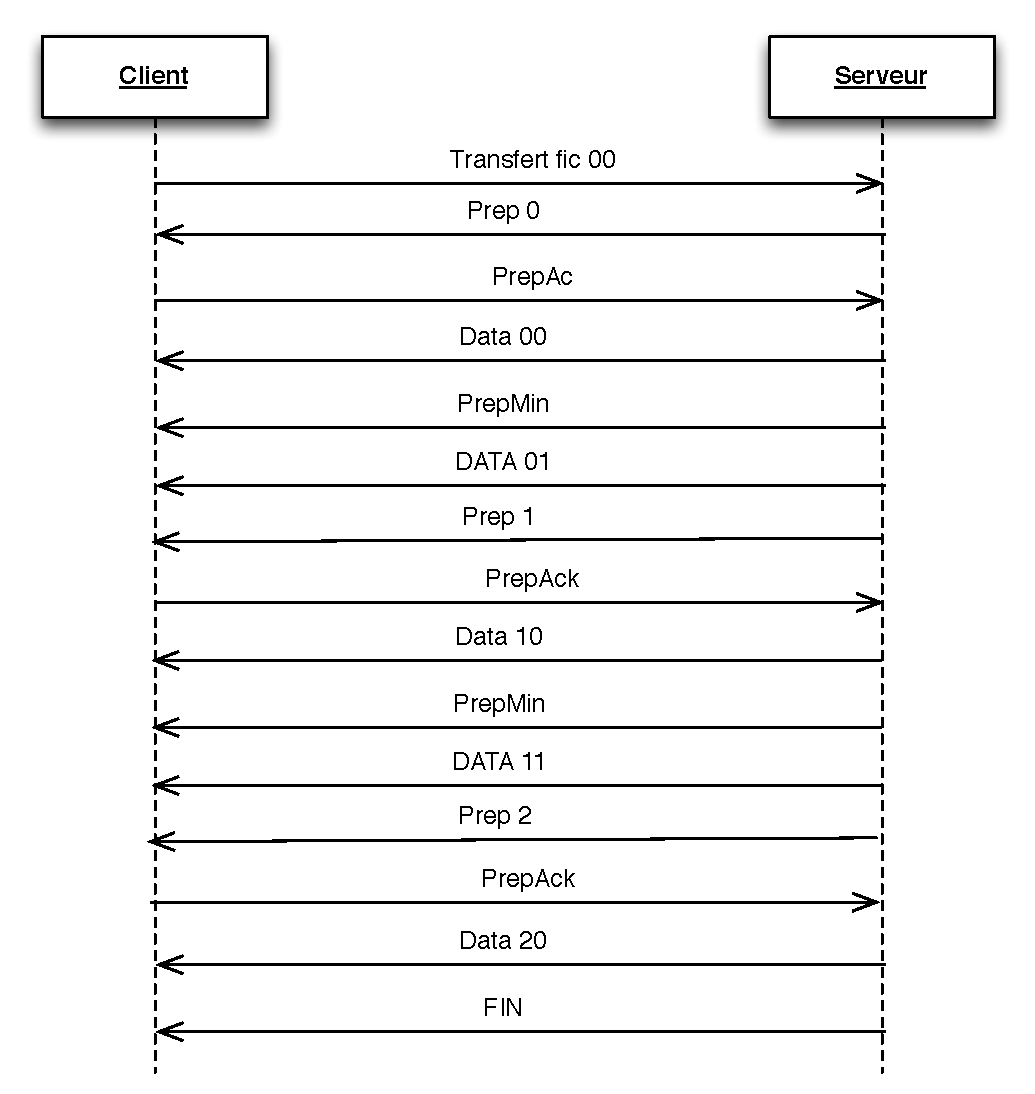
\includegraphics[width=10cm, height=13cm]{graphics/Diag_seq.pdf}
\end{center}
	\caption{Diagramme de s�quence 2 - Q5}
	\label{fig:Diag_seq}
\end{figure}

\newpage

\subsection{En utilisant les primitives de la question pr�c�dente, �crire le pseudo-code ou le code Java des primitives client(fic,i,j) et serveur()}

\begin{verbatimtab}
client(fic,i,j) {
	String msg;
	OuvrirCx(Serveur);
	attendreCx();
	envoyer("TRANSFERT "+fic+ " "+i+ " "+j);
	
	
	processMess(mes);
	
	while ((mes = recevoir()) != "FIN") {
		if (msg == "Prep") {
			// stocker i;
			envoyer("PrepAck");
		} else if (msg == "PrepMin") {
			// stocker j
		} else if (msg == "DATA" ){
			// stocker dans n fichier
		}
	}
	
	fermerCx();
}

envoyerFichier(String fic) {
	int nb = nbBloc100K(fic);
	int prep = 0,  j = 0;
	
	for (int i = 0; i< nb ; i++) {
		if (i\%2 == 0) {
			envoyer("Prep" prep++);
			recevoir(); // pour ack
			j = 0
		}
		else {
			envoyer("PrepMin");
			j = 1;
		}
		emvoyer ("DATA"+i+" "+j);
	}
}

\end{verbatimtab}


\end{document}